\chapter{Testy}
\label{cha:testy}

Poniżej prezentujemy testy jakie przeprowadzliśmy wraz z ich krótkim opisem oraz niezbędnymi zmianami w kodzie oraz komentarzem odnoszącym się do rezultatów otrzymywanych z w3af.

\section{Click-Jacking}
\begin{enumerate}
\item Opis podatności\\
CLick-Jacking to złośliwa technika nakłaniające użytkowników do klikania w inne rzeczy niż oni sami myślą, że klikają.
Może dojść do potencjalnego ujawnienia poufnych inforamcji lub przejęcia kontroli nad ich komputerem, po kliknięciu na pozornie niewinną stronę. Click-jacking przybiera też formę wbudowanego kodu lub skryptu, który może został wywołany bez wiedzy użytkownika.
\item Zmiany w kodzie\\
Nie były wymagane w przypadku tej podatności.
\item Komentarz\\
W3AF podczas pierwszego uruchomienia, bez zmian w kodzie, wykrył podatność aplikacji Moodle na brak zabezpieczeń przed atakami click-jacking. 
\end{enumerate}

\noindent
\begin{minipage}{\linewidth}
\makebox[\linewidth]{
  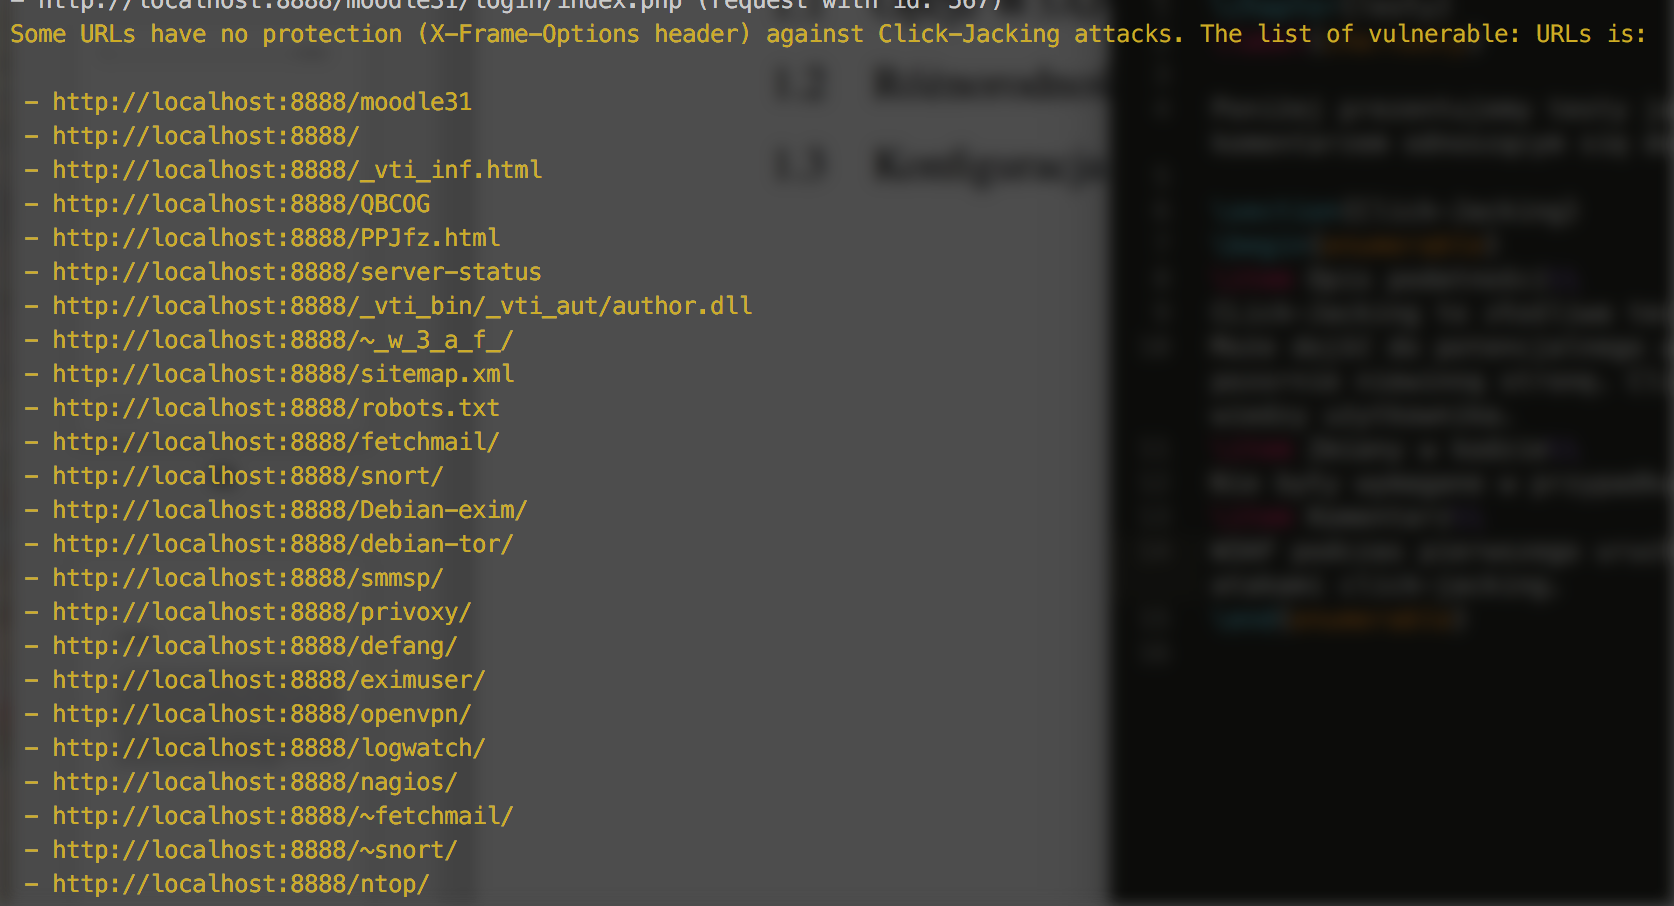
\includegraphics[keepaspectratio=true,scale=0.5]{pictures/clickjacking.png}}
\captionof{figure}{Wyniki W3AF dotyczące clickjackingu}\label{erd}
\end{minipage}

%--------------------------------------

\section{CSRF}
\begin{enumerate}
\item Opis podatności\\
CSRF - metoda ataku na serwis internetowy, która często (m.in. na skutek jednoczesnego wykorzystania) mylona jest z cross-site scripting (XSS) bądź jest uznawana za jej podzbiór. Ofiarami CSRF stają się użytkownicy nieświadomie przesyłający do serwera żądania spreparowane przez osoby o wrogich zamiarach. W przeciwieństwie do XSS, ataki te nie są wymierzone w strony internetowe i nie muszą powodować zmiany ich treści. Celem crackera jest wykorzystanie uprawnień ofiary do wykonania operacji w przeciwnym razie wymagających jej zgody. Błąd typu CSRF dotyczy również serwerów FTP. 
\item Zmiany w kodzie\\
Nie były wymagane w przypadku tej podatności.
\item Komentarz\\
W3AF znalazł podatność na CSRF podczas pierwszego uruchomienia testów:
\noindent
\begin{minipage}{\linewidth}
\makebox[\linewidth]{
  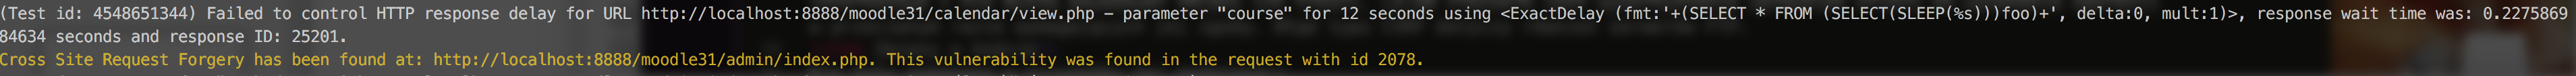
\includegraphics[keepaspectratio=true,scale=0.3]{pictures/csrf.png}}
\captionof{figure}{Wyniki W3AF dotyczące cross site request forgery}\label{erd}
\end{minipage}
\end{enumerate}


%--------------------------------------

\section{SQL injection}
\begin{enumerate}
\item Opis podatności\\
 metoda ataku komputerowego wykorzystująca lukę w zabezpieczeniach aplikacji polegającą na nieodpowiednim filtrowaniu lub niedostatecznym typowaniu danych użytkownika, które to dane są później wykorzystywane przy wykonaniu zapytań (SQL) do bazy danych. Podatne są na nią wszystkie systemy przyjmujące dane od użytkownika i dynamicznie generujące zapytania do bazy danych.
\item Zmiany w kodzie\\
Nie były wymagane w przypadku tej podatności.
\item Komentarz\\
W3AF, a konkretnie plugin blind\_sqli znalazł podatność na CSRF podczas pierwszego uruchomienia testów. Podatne na atak SQL injection są miejsca wpisywania loginu i hasła przez użytkownika.
\noindent
\begin{minipage}{\linewidth}
\makebox[\linewidth]{
  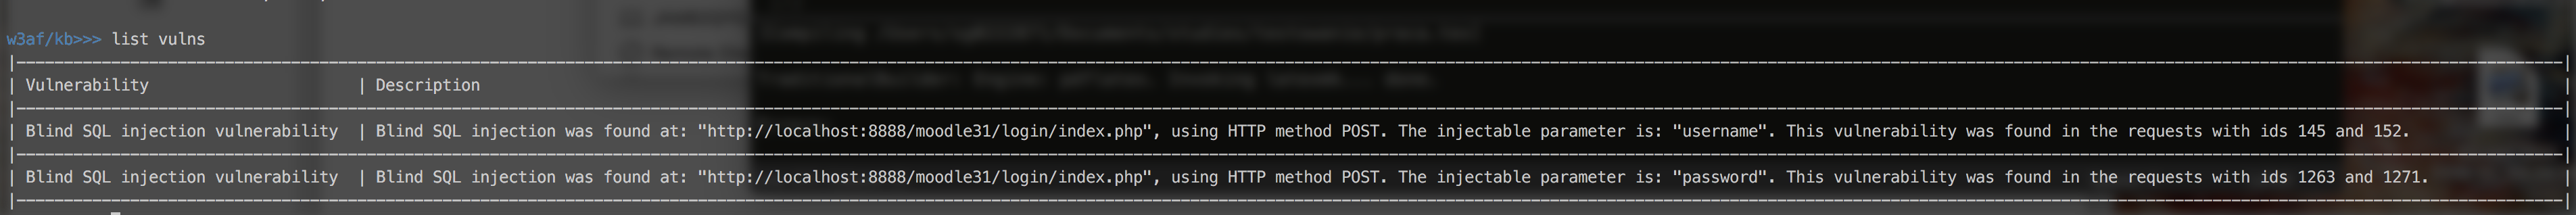
\includegraphics[keepaspectratio=true,scale=0.3]{pictures/sqli.png}}
\captionof{figure}{Wyniki W3AF z bazy wiedzy na temat sql injection}\label{erd}
\end{minipage}
\end{enumerate}
